\documentclass{article}
\usepackage{icmc,amsmath}
\usepackage{graphicx}
\usepackage{url}
\usepackage[utf8x]{inputenc}
\usepackage[english]{babel}
\usepackage{color}
\usepackage[htt]{hyphenat}
\usepackage{babelbib}

\title{Rameau: A System for Automatic Harmonic Analysis}

\oneauthor
  {Pedro Kröger, Alexandre Passos, Marcos Sampaio, Givaldo de Cidra}
  {Genos---Computer Music Research Group\\ School of Music
   \\ Federal University of Bahia, Brazil \\
  \url{{pedro.kroger,alexandre.tp,mdsmus,givaldodecidra}@gmail.com}}

\newcounter{notacounter}

\newcommand{\nota}[1]{
  \addtocounter{notacounter}{1}
  \textcolor{red}{[nota \arabic{notacounter}: #1]}
}


\begin{document}
\graphicspath{{figs/}{data/}}
\maketitle

\begin{abstract}
%The abstract should be placed at the top left column and should contain
%about 150-200 words.

\end{abstract}

\section{Introduction}
\label{sec:introduction}

In music, harmonic analysis is the study of vertical sonorities and it
connections and is paramount to the understanding of tonal
compositions. The analyst may find the root of chords, label
sonorities with proper chords names (such as ``A minor''), and
identify the relationship between chords using roman
numerals.

Harmonic analysis by computer is an important, challenging, and
interesting computer music research topic. It is challenging because
the musical material has a large variety of information such as
timbre, notes, rhythm, dynamics, harmony, and by the fact that music
is not a linear process, unlike image \cite{mouton.ea:numeric}. The
harmonic changes in a choral texture, where usually all notes in all
voices begin and finish at the same time, are obvious. However, chords
are ocasionally arppeggiated, incomplete, and intertwined with
non-harmonic tones. These things contribute to increase considerably
the complexity for analysis \cite{pardo.ea:automated}.

There are many practical applications for automatic music analysis,
among them arranging, detection of possible logical mistakes in
scores, database search, automatic accompaniment generation, and
statistical analysis of musical styles for automated composition
\cite{pardo.ea:algorithms,temperley.ea:modeling}. Computer-based
harmonic analysis is also important because it can bring new insights
in music theory, in the same way the use of computer in vision and
problem solving has brought new insights in these areas
\cite{temperley.ea:modeling}. 

Until now a single framework that allows comparison between different
algorithms and analysis results has not been developed. Pardo and
Birmingham state that ``no researchers have published statistical
performance results on a system designed to analyze tonal music''
\cite{pardo.ea:algorithms} before their paper. This lack of data in
literature makes it difficult to compare different systems. Also,
there aren't standard benchmarks to compare different algorithms and
analysis results. In fact, only Pardo and Birmingham
\cite{pardo.ea:automated} and Barthèlemy and Bonardi
\cite{barthelemy.ea:figured} published specific comparisons between
different analysis results. Pardo and Birmingham compare their results
with Temperley and Sleator's \cite{temperley.ea:modeling} while
Barthèlemy compares his model against Maxwell's, Pardo and
Birmingham's, and Temperley and Sleator's
\cite{maxwell:expert,temperley:algorithm,pardo.ea:automated}. However,
these comparisons are based on results published in papers and not
from direct implementations, so they aren't statistically
representative. Tsui \cite{tsui:harmonic} gives a general comparisson
of his algorithm with Taube's \cite{taube:automatic} and Temperley's
\cite{temperley:algorithm}. Unfortunatelly the results of
\cite{taube:automatic} are not published in the paper but in a web
site that is no longer on-line, making further comparisson impossible.
Illescas et al. \cite{illescas.ea:harmonic} have a even more general
comparison with \cite{taube:automatic} where their system ``is
comparable in results to those reported by MTW [Taube's system]''.

The systems of Illescas et al. \cite{illescas.ea:harmonic} and Raphael
and Stoddard \cite{raphael.ea:harmonic} don't show the inversion of
chords, differentiate major from minor chords (they print both in
upper case), and provide objective results, such as error rates or
accuracy degree.

To the best of our knowledge, \cite{illescas.ea:harmonic} and
\cite{taube:automatic} are the only systems that provide non-chord
tone (NCT) analysis. \cite{taube:automatic} prints the type of the NCT
bellow the note, using PT for passing tone, NT for neighbor tone, and
so on, while \cite{illescas.ea:harmonic} prints a very detailed
analysis for each NCT.

Barthèlemy \cite{barthelemy.ea:figured} provides a good sumary of the
state of the art of harmonic analysis up to 2001.

In this paper we present Rameau, a framework for automatic harmonic
analysis of Western tonal music. We also present an preliminary
evaluation of nine algorithms for harmonic analysis, using a corpus of
140 Bach Chorales from the Riemenschneider edition. Section
\ref{sec:system} describes Rameau in more details, section
\ref{sec:problem} lists the problems related to harmonic analysis,
section \ref{sec:analysis-results} analyses the results obtained, and
section \ref{sec:concl-future-work} .......

\section{The problem of automated harmonic analysis}
\label{sec:problem}

The problem of automated harmonic analysis might be understood by
dividing it into four sub-problems. 

The first problem is pitch spelling. If sharps and flats are not
distinguished the program may have problems in places where enharmonic
information is important. Most systems either ignore this problem or
develop a pitch speller \cite{temperley.ea:modeling}. To our knowledge
most harmonic analysis software (with the notable exception of the
MusEs \cite{pachet.ea:representing} system) uses input formats that
lose enharmonic information.

The second problem, the segmentation problem
\cite{pardo.ea:automated}, is determining what are the vertical
sonorities in a piece of music and grouping these sonorities into
harmonically significant segments, or chord-spans. Most of the
difficulty of segmenting is due to the number of possible
segmentations of a piece being roughly an exponential function of its
length \cite{pardo.ea:algorithms}.

The third problem is labeling segments with chord names. Not every
segment forms a chord, though---some will consist solely of non-chord
tones and other melodic information. Labeling a segment with a chord might
require contextual information, which complicates the matter a bit,
difficulting local decisions. Still, over 80\% of accuracy is possible
ignoring context (see section \ref{sec:analysis-results}).

The last problem is finding the main key and the modulations of the
piece and assigning a tonal function to each chord.

\section{Numeric codification for tonal music}
\label{sec:codificacao-jamary}

Probably the pitch-class notation, or some variation such as MIDI, is
the most used way to numerically represent pitch. The main problem
with this notation is the loss of enharmonic spelling. In this section
we will revise three notations created independently by Brinkman,
Hewlett, and Oliveira \cite{brinkman:binomial,
  hewlett:base-40, oliveira:busca} to address this problem.
For simplicity we will refer to them as binomial, base-40, and
base-96, respectively.

Notes in the binomial notation are represented as tuples in the form
of \texttt{<pc,nc>} where \texttt{pc} stands for pitch-class and
\texttt{nc} for note-class. Note-class is a modulo 7 notation system
that represents numerically each note name (A, B, C, D, E, F, G) from
0 to 6. 0 represents any C, with or without accidentals, 1 represents
any D, with or without accidentals, and so on. For example, C$\sharp$
is represented as \texttt{<1,0>}, D$\flat$ as \texttt{<1,1>}, and C$\flat$
as \texttt{<11,0>}. In this last example 11 represents the pich-class of the
note and 0 indicates how it will be spelled. The binomial notation
also allows a packaged representation using only single numbers, where
the pitch-class is multiplied by 10 and added to the note-class. For
example, C$\sharp$ becomes 10 and D$\flat$ 11.

Unlike the binomial notation, the base-40 notation uses only single
numbers. The octave is divided linearly in 40 notes from C$\flat\flat$
to B$\sharp\sharp$. Table \ref{tab:base40} shows a few notes in this
system.

\begin{table}
  \centering
  \begin{tabular}{l|l}
    note & code \\
    \hline
    c$\flat\flat$ & 1 \\
    c$\flat$ & 2 \\
    c & 3 \\
    c$\sharp$ & 4 \\
    c$\sharp\sharp$ & 5 \\
    -- & 6 \\
  \end{tabular}
  \caption{A few notes in the base-40 notation}
  \label{tab:base40}
\end{table}

The base-96 notation is simple, elegant, and overcomes a few
shortcommings in both the binomial and base-40 notations. Since the
original publication of the base-96 notation is available only in
Portuguese, we will describe it here, comparing with the other
two.

The base-96 is also a single number notation. It has all the
advantagens of the base-40 notation with a few advantagens. Table
\ref{tab:jama-notas} shows how notes are encoded. In this notation the
intervals are invariant under most transformations, such as inversion,
transposition, etc. Table \ref{tab:jama-intervalos} shows the coding
for the intervals. In this table the first column indicates the
interval name; p, M, m, d, A for perfect, major, minor, diminished,
and augmented, respectively. The letters before d and A indicate the
quantity of the interval. For instance, tA is triple-augmented.

\begin{table}
  \centering
  \begin{tabular}{l|lllllll}
               & c & d& e& f& g& a& b \\
    \hline
    7$\flat$   &   & 7&21&  &  &62&76 \\
    6$\flat$   & 90& 8&22&35&49&63&77 \\
    5$\flat$   & 91& 9&23&36&50&64&78 \\
    4$\flat$   & 92&10&24&37&51&65&79 \\
    3$\flat$   & 93&11&25&38&52&66&80 \\
    2$\flat$   & 94&12&26&39&53&67&81 \\
    $\flat$    & 95&13&27&40&54&68&82 \\
    $\natural$ &  0&14&28&41&55&69&83 \\
    $\sharp$   &  1&15&29&42&56&70&84 \\
    2$\sharp$  &  2&16&30&43&57&71&85 \\
    3$\sharp$  &  3&17&31&44&58&72&86 \\
    4$\sharp$  &  4&18&32&45&59&73&87 \\
    5$\sharp$  &  5&19&33&46&60&74&88 \\
    6$\sharp$  &  6&20&34&47&61&75&89 \\
    7$\sharp$  &   &  &  &48&  &  &   \\
  \end{tabular}
  \caption{Notes in the base-96 notation}
  \label{tab:jama-notas}
\end{table}

\begin{table}
  \centering
  \begin{tabular}{l|llllllll}
    & 1$^{st}$& 2$^{nd}$& 3$^{rd}$& 4$^{th}$& 5$^{th}$& 6$^{th}$& 7$^{th}$& 8$^{th}$ \\
    \hline
    sd  &  & 7&21&35&49&62&76&90 \\
    qd  &  & 8&22&36&50&63&77&91 \\
    qd  &  & 9&23&37&51&64&77&92 \\
    td  &  &10&24&38&52&65&78&93 \\
    dd  &  &11&25&39&53&66&79&94 \\
    d   &  &12&26&40&54&67&80&95 \\
    m   &  &13&27&  &  &68&82&   \\
    P   & 0&  &  &41&55&  &  &96 \\
    M   &  &14&28&  &  &69&83&   \\
    A   & 1&15&29&42&56&70&84&   \\
    dA  & 2&16&30&43&57&71&85&   \\
    tA  & 3&17&31&44&58&72&86&   \\
    qA  & 4&18&32&45&59&73&87&   \\
    qA  & 5&19&33&46&60&74&88&   \\
    sA  & 6&20&34&47&61&75&89&   \\
    oA  &  &  &  &48&  &  &  &   
  \end{tabular}
  \caption{Invervals in base-96 notation}
  \label{tab:jama-intervalos}
\end{table}

The base-96 notation works for up to seven flats and sharps, which is
more than enough for tonal music. This system is compatible with the
pitch-class system (modulo 12): in the base-96 notation G = 55, and
the result of 55 mod 12 is 7, representing G in the pitch-class
notation. 

The problem with the base-40 notation is that it has problems with
more than two accidentals. For example, the interval between
C$\flat\flat$ and C$\sharp\sharp$ (a quadruple augmented unison) has
the same value (6) as diminished second. On the other hand, in the
base-96 notation this interval can be correctly computed.

The main problem with the binomial notation is that operations that
are (and should be) simple become complex. In both base-40 and base-96
notations, transposition is as simple as adding an index to a note, while
in the binomial system it has to use two different operations (mod and
div) besides the addition. Its packaged representation is supposed to
simplify things, but as an example, transposition become something
like:

\begin{eqnarray}
10\times((a \div 10 + B \div 10) \mod 12)\; + \nonumber \\
((a \mod 10 + B \div 10) \mod 7)
\end{eqnarray}

To do anything non-trivial, like interval-class vectors, yet extra
work has to be done, increasing complexity.

 believe the base-96 codification is a very nice form of describing
tonal music numerically and it should be more known among researches
and developers. For these reasons we have adopted it, although no
algorithm at present makes direct use of it, since their original
authors designed them expecting pitch classes as input. \nota{passos:
  corrigido o problema? kroger: eu acho que precisamos deixar mais
  claro a ideia de que estamos re-implementando outros algor.}

\section{The Rameau Framework}
\label{sec:system}

To properly study, understand and compare algorithms for automated
harmonic analysis we have designed and implemented a framework,
Rameau, that should enable us to

\begin{enumerate}
\item compare results precisely and repeatably with human analysis of
  a large corpus of music;
\item allow algorithms to access detailed information in the input score,
  such as enharmonic differences, meter, etc.; and
\item easily develop new algorithms, test existing ones, and precisely
  compare the results.
\end{enumerate}

Reimplementing existing algorithms in Rameau allows us to easily
evaluate their accuracy, study their errors and compare them with our
baseline techniques. We are unaware of research comparing different
approaches for harmonic analysis, in the manner of reference
\cite{gomez.ea:song}.

Rameau is written in Common Lisp and runs on the Steel Bank Common
Lisp \cite{team:sbcl} compiler on the GNU/Linux operating system.
\nota{run, run, run!} Rameau also runs on windows (it might run on
MacOS, but that was not tested) and is portable enough to be compiled
with CMUCL \cite{maclachlan:cmucl} and Clisp \cite{haible.ea:clisp}.

\subsection{Architecture}
\label{sec:architecture-and-api}

The architecture of the Rameau framework is simple. First, a score is
parsed (our parser is written using Cl-Yacc
\cite{chroboczek:cl-yacc} and Cl-Lexer
\cite{parker:lexer}) into a list of notes, which is then split
into a list of sonorities. Then, these sonorities are sent to each
algorithm for analysis. The analysis results and their comparison with
the answer sheets are then output either textually or as an annotated
score, as in figures \ref{fig:coral-12} and \ref{fig:coral-54}.

The algorithms used for analysis are implemented using a very simple
Common Lisp API. To implement one it is enough to place a lisp file in
a special directory and call the \texttt{register-algorithm} function
inside that file, specifying the algorithm's name, an analysis
function and a comparison function as parameters. The input to the
analysis function is a list of sonorities. In Rameau, sonorities are
lists of notes, each note specifying its onset time, duration, octave
and pitch. The output is a list of either chords or non-chord tones,
one for each input sonority. Chords are structures possibly having a
root, a mode, a seventh, a bass, and other additions. The
framework provides a few possible comparison functions for easy
usage.

We have currently implemented using this API 
\begin{enumerate}
\item a subset of the algorithm described in \cite{pardo.ea:algorithms}
  (ignoring, for now, segmentation), 
\item a work-in-progress port of the algorithm described in
  \cite{temperley.ea:modeling}, 
\item four neural networks (using the Fann \cite{nissen:fann}
  library) roughly similiar to some described in
  \cite{tsui:harmonic}, and
\item four decision trees modeled after the neural networks (using code
  from \cite{mitchell:machine}).
\end{enumerate}

Rameau's source code is publicly available, under a GNU GPL
\cite{fsf:gpl} license in a git \cite{baudis:git}
repository at \url{genos.mus.br/repos/rameau.git} and for
visualization at \url{git.genos.mus.br/?p=rameau.git}.

\subsection{The interface}
\label{sec:analysis-output}

Rameau is a command line program, although a GUI version is planned.
The user can select the chorales to be analyzed and specify the
algorithms for the analysis. The output shows a table with the
partition number, the correct analysis for each sonority (taken from
the answer sheet) and the analysis output for each chosen algorithm.
The nice thing about this output is that it can be further processed
using regular unix tools such as grep, awk, and sed.

To simplify reading for humans, rameau can output a score with the
chorale and the analysis from each algorithm chosen. The music
notation program LilyPond \cite{nienhuys.ea:lilypond} is used to
render the score.

Figure \ref{fig:coral-12} shows the result of the analysis of the
first phrase of chorale \#12. The first line shows the partition
number, the last line the expected answer, and the lines in between
the analysis results for the chosen algorithms. The output score shows
incorrect analysis in bold italic. Non-chord tones are notated as
``—''. It is important to remember that while some algorithms identify
chords, others identify only the root.

\begin{figure}
  \centering
  \includegraphics[scale=4]{coral-012}
  \caption{An analysed excerpt from chorale 12, ``Puer natus in Bethlem''}
  \label{fig:coral-12}
\end{figure}

\subsection{Test corpus}
\label{sec:test-corpus}

We are building a corpus of analyzed and digitalized Bach chorales to
use as training and test data. Bach chorales were chosen because:

\begin{enumerate}
\item they are easily analyzed. For example, the segmentation problem in
them consists simply of determining the sonorities.
\item Their chord density is high - there are many more chords per
  measure than in a symphony, for example.
\item They are canonical examples of tonal harmony.
\item There are 371 on the Riemenschneider edition, more than
  enough to train our algorithms and get precise error analysis.
\item Their texture is simple and constant. It consists basically of
  four voices forming simple triads and tetrads.
\end{enumerate}

We have already analyzed 140 of them and plan on fully analyzing the
Riemenschneider corpus soon. The chorales are stored in a subset of
the GNU Lilypond \cite{nienhuys.ea:lilypond} format, from which we
generate MIDI files and typeset scores, possibly annotated with
analysis results (both by human and by computer).

When the chorales are fully analysed we plan on incorporating the
Kostka-Payne \cite{kostka.ea:tonal} corpus, Beethoven sonatas, Bach
cello suites and other pieces.

\subsection{The answer sheet format}
\label{sec:formato-dos-acordes}

The results of human analysis performed on the chorales are stored in
a simple, flexible text format, designed to

\begin{enumerate}
\item be as close as possible to usual popular notation,
\item represent inherent ambiguities in chord, and
\item single out sonorities that do not constitute chords, instead
  having melodic functions on the piece.
\end{enumerate}

The first four sonorities of the answer sheet for Bach's chorale \#1
``Aus meines Herzens Grunde'', for example, are stored as \texttt{G G
  C/E (C7+/E [b])}. Each chord symbols represents a sonority. Chords
in parenthesis represent possible interpretations of a single
sonority. Notes in brackets are non-chord tones, marking sonorities
that do not constitute chords.

This information is then used as answer sheets and training data on the
many algorithms implemented in our system.

\section{Preliminary results}
\label{sec:analysis-results}

\subsection{Pardo and Birmingham's algorithm}
\label{sec:pardo-birmingham}

The algorithm described in \cite{pardo.ea:automated} has some
interesting properties. It handles most simple examples of tonal
harmony really well, but has no clear notion, by design, of non-chord
tones, augmented chords and other possible analysis. We
have found no need, as of yet, of implementing the segmentation
algorithm, since segmentation is trivial in Bach Chorales.

The current accuracy is $66 \pm 9\%$.


\subsection{Neural networks}
\label{sec:neural-nets}

Neural networks are tools for non-linear statistical data
modeling that work by having artificial neurons exchange
information. There are many varieties of neural networks, each being
useful for a certain type of problem. Our networks are all multilayer
feedforward neural networks, with one hidden layer each. This is the
standard model for pattern recognition \cite{russell.ea:artificial}.

A neural network is made of connected neurons. Each neuron receives
signals from other neurons, processes them in a simple manner and
forwards them to yet other neurons, as in figure \ref{fig:neuron}. In
a feedforward neural network, these signals flow linearly from input
neurons to output neurons. We use feedforward neural networks in which
the neurons are arranged in layers, as in figure
\ref{fig:simple-net-diagram}. Each neuron receives information from
all neurons in the layer preceding it and forwards information to all
neurons in the next layer. The first layer, the input layer, receives
the input to the neural network as information, and the output layer
emits the neural network's outputs. One hidden layer between the input
and output layers is enough to represent every continuous function
with arbitrarily small error \cite{russell.ea:artificial}. How each
individual neuron will process its input is determined by training,
usually with the backpropagation algorithm or a variant of it.


\begin{figure}
  \includegraphics[scale=1]{neuron}
  \caption{A single neuron in a neural network}
  \label{fig:neuron}
\end{figure}

\begin{figure}
  \includegraphics[]{neural-networks}
  \caption{The Simple-net}
  \label{fig:simple-net-diagram}
\end{figure}


We have currently implemented in Rameau four neural-network-based
algorithms for harmonic analysis, basing our approaches on
\cite{tsui:harmonic}. The input of our simplest algorithm,
\texttt{Simple\hyp{}net}, is how many times each pitch class sounds in
a sonority (its pitch count). As output, the network activates the
neuron representing the root for that sonority (or does nothing, if
the sonority does not form a chord). Figure
\ref{fig:simple-net-diagram} illustrates its connections and labels.
To study the effect of contextual information in harmonic analysis we
have also implemented \texttt{Context-net}, differing from the
\texttt{Simple\hyp{}net} only by also looking at the pitch counts of
two preceding sonorities and one immediately the one being analysed.
\texttt{Context-net} and \texttt{Simple-net}'s performances are
equivalent, so perhaps the contextual information necessary for
harmonic analysis is not easily inferrable from pitch counts. The two
other neural networks, \texttt{Chord-net} and \texttt{Mode-net}, also
determine a chord's mode and its seventh. \texttt{Chord-net}'s input
is the same as \texttt{Sim\-ple\--net}'s, while \texttt{Mode-net} also
sees the results of \texttt{Context-net}'s analysis for each sonority.

The performance of each neural network depends heavily on the number
of hidden units it uses. Too few units and the network hasn't got
enough memory to learn enough harmonic patterns. Too many, and the
network faces the risk of overfitting. Overfitting happens when the
neural network has too much memory, so it starts inferring inexistent
patterns from noise in the training data. This is similar to a
superstitious person's belief that some things bring ``good luck'' or
``bad luck'', according to \cite{white.ea:superstitious}.

The ideal number of hidden units in a neural network has to be
determined experimentally. The experiments for each of our networks
can be seen figures \ref{fig:simple-net}, \ref{fig:context-net},
\ref{fig:chord-net}, and \ref{fig:mode-net}. The chosen values were 12
units for \texttt{Sim\-ple\--net}, 24 for \texttt{Context-net}, 55 for
\texttt{Chord-net} and 50 for \texttt{Mode-net}.

Our current accuracies for these algorithms are $88\pm 8\%$ for
\texttt{Simple-net}, $87 \pm 8\%$ for \texttt{Context-net}, $83 \pm
8\%$ for \texttt{Chord-net} and $83 \pm 8\%$ for \texttt{Mode-net}.

\begin{figure}
  \includegraphics[scale=0.35,angle=270]{dados-simple-net}
  \caption{Accuracy versus number of hidden nodes in the simple-net}
  \label{fig:simple-net}
\end{figure}

\begin{figure}
  \includegraphics[scale=0.35,angle=270]{dados-context-net}
  \caption{Accuracy versus number of hidden nodes in the context-net}
  \label{fig:context-net}
\end{figure}

\begin{figure}
  \includegraphics[scale=0.35,angle=270]{dados-chord-net}
  \caption{Accuracy versus number of hidden nodes in the chord-net}
  \label{fig:chord-net}
\end{figure}

\begin{figure}
  \includegraphics[scale=0.35,angle=270]{dados-mode-net}
  \caption{Accuracy versus number of hidden nodes in the mode-net}
  \label{fig:mode-net}
\end{figure}

\subsection{Decision trees}
\label{sec:decision-trees}

Decision trees are useful data modeling tools, with many uses in the
machine learning community \cite{mitchell:machine,
  russell.ea:artificial}. They are most useful when trying to extract
meaningful patterns from data in a human-readable way. We have built
four decision trees that perform harmonic analysis, each mirroring one
of the neural networks. \texttt{Simple-tree} looks at the pitches in a
sonority and outputs the sonority's root. \texttt{Context-tree} looks
also at the pitches in a few surrounding
sonorities. \texttt{Chord-tree} looks at the pitches of a sonority and
outputs its mode. \texttt{Mode-tree} looks at the pitches of a
sonority (transposed to match \texttt{Simple-tree}'s analysis for that
sonority) and outputs only the mode, which is matched with
\texttt{Simple-tree}'s root to get a result.

Our current accuracies for the decision-tree based algorithms are $82
\pm 8\%$ for \texttt{Simple-tree}, $76 \pm 9\%$ for
\texttt{Context-tree}, $77 \pm 10\%$ for \texttt{Mode-tree} and $50
\pm 11$ for \texttt{Chord-tree}.

\subsection{The effect of training set size}

The effect training set size on the accuracy of the neural networks
and decision trees can be seen in figure
\ref{fig:treinamento-corais}. One chorale is enough information for
\texttt{Simple-net}, and most decision-tree algorithms need far more
chorales than their neural-network counterparts to perform similarly,
due to their lower generalization performance.

\begin{figure}
  \includegraphics[scale=0.35,angle=270]{treinamento-corais}
  \caption{Accuracy versus amount of training data per algorithm}
  \label{fig:treinamento-corais}
\end{figure}


\subsection{Performance analysis}
\label{sec:common-errors}

We believe a more systematic study of the errors made by harmonic
analysis methods is necessary to understand and improve them. Since
harmonic analysis can be seen as an information retrieval problem,
metrics developed to assess the performance of information retrieval
systems should help understanding and evaluating the performance of
harmonic analysis algorithms. For this reason we chose to analyze our
results in terms of precision and recall. Precision measures how
correct are the returned results, while recall measures how likely is
a sonority's mode to be correctly recognized, as can be seen in the
chapter 23 of \cite{russell.ea:artificial}. While a combined measure
of these characteristics (like average accuracy over all sonorities)
is a good assessment of the general performance of an algorithm, it
hides a lot of interesting information on its behavior.

Tables \ref{tab:precision} and \ref{tab:recall} show that with proper
modifications to classify more chord modes Pardo and Birmingham's
algorithm can match or even exceed the accuracy of our current machine
learning techniques. Table \ref{tab:recall} shows that our machine
learning algorithms are missing many melodic notes. Tables
\ref{tab:precision} and \ref{tab:recall} indicate that the neural
network algorithms are failing to recognize fully diminished,
incomplete, and augmented chords, probably because that our training
corpus lacks enough examples of these chords, as seen in table
\ref{tab:frequency}. Because the decision trees are better at these
rare chords we can conclude that they recall few examples better,
while the neural networks tend to generalize more efficiently when
more examples are available.

As we implement more algorithms, performance analysis by rigorous
metrics will enable us to draw better conclusions as to the merits and
flaws of each technique.


\begin{table}
  \centering
  \begin{tabular}{l|p{.1cm}p{.1cm}p{.1cm}p{.1cm}p{.1cm}p{.1cm}p{.1cm}p{.1cm}p{.1cm}p{.1cm}p{.25cm}|p{.1cm}}
                 &  °& °7& ø7& m&  m7&  M&  7& 7+&+&nct&inc& avg\\
    \hline                                                     
    Pardo-Birm   & 63& 59& 37& 77&  0& 66& 72&  0&0&  0&  0& 34 \\
    Mode tree    & 56& 54& 66& 78& 61& 87& 76& 27&0& 85& 23& 56 \\
    Chord tree   & 56& 54& 66& 78& 67& 87& 76& 27&0& 85& 23& 56 \\
    Mode net     & 67&  0& 72& 89& 70& 92& 85& 34&0& 84&  0& 54 \\
    Chord net    & 70&  0& 71& 87& 75& 90& 89& 35&0& 86& 18& 56 \\
  \end{tabular}
  \caption{Precision (\%)}
  \label{tab:precision}
\end{table}

\begin{table}
  \centering
  \begin{tabular}{l|p{.1cm}p{.1cm}p{.1cm}p{.1cm}p{.1cm}p{.1cm}p{.1cm}p{.1cm}p{.1cm}p{.1cm}p{.25cm}}
    Chord        &  °& °7& ø7&   m& m7&   M&  7& 7+&+  & nct&inc \\
    \hline                                                     
    Frequency    &2.8&0.7&2.3&16.4&4.6&37.6&9.6&1.0&0.1&24.3&0.3  \\
  \end{tabular}
  \caption{Frequency of chords in our corpus (\%)}
  \label{tab:frequency}
\end{table}


\begin{table}
  \centering
  \begin{tabular}{l|p{.1cm}p{.1cm}p{.1cm}p{.1cm}p{.1cm}p{.1cm}p{.1cm}p{.1cm}p{.1cm}p{.1cm}p{.25cm}|p{.1cm}}
                 &  °& °7& ø7& m&  m7&  M&  7& 7+&+&nct& inc& avg\\
    \hline
    Pardo-Birm   & 86& 85& 77& 91&  0& 97& 93&  0&  0&  0&  0& 48 \\
    Mode tree    & 68& 36& 44& 89& 65& 94& 82& 59&  0& 55& 18& 55 \\
    Chord tree   & 68& 37& 45& 88& 66& 94& 82& 56&  0& 58& 18& 56 \\
    Mode net     & 81&  0& 61& 93& 82& 94& 90& 70&  0& 68&  0& 58 \\
    Chord net    & 86&  0& 68& 93& 77& 95& 88& 78&  0& 67&  5& 60 \\
  \end{tabular}
  \caption{Recall (\%)}
  \label{tab:recall}
\end{table}

\begin{figure}
  \centering
  \includegraphics[scale=4]{coral-054}
  \caption{An analysed excerpt from chorale 54, ``Lobt Gott, ihr
    Christen, allzugleich''}
  \label{fig:coral-54}
\end{figure}

\subsection{Analysis example}
\label{sec:analysis-example}

The chorale exerpt in figure \ref{fig:coral-54} is a little tricky to
analyse because the all chords in partitions 36--39 have a non-chord
tone. The A in partition 36 as a retardation, the C in p. 37 a
passage, the G in p. 38 another retardation, and the E in p. a
cambiata. It is interesting to observe that the neural network based
algorithms identify correctely the non-chords tones, the decision tree
algorithms fail in partitions 36 and 37 but give a correct answer in
p. 38--39, pardo-birmingham is able to indentify the basic harmonic
framework (without non-chord tones, however), while temperley-sleator
incorrectelly assumes all chords have G as root.

\section{Conclusions and future work}
\label{sec:concl-future-work}

In this article we described Rameau, a framework for studying
automatic harmonic analysis of tonal music.

Right now our research can branch in many directions. A few important
algorithms, like Maxwell's expert system \cite{maxwell:expert},
Ulrich's algorithm \cite{ulrich:analysis}, a variant of Noland and
Sandler's Hidden Markov Model-based key-finding algorithm
\cite{noland.ea:key}, and many others are still unimplemented. We plan
on implementing segmentation and functional analysis, which will allow
us to extend our corpus, incorporating, for example, the KP corpus
\cite{temperley:bayesian}. We are also looking for new metrics and
evaluation techniques, and will extend and improve our existing
algorithms accordingly. We believe all these tasks will be
considerably easier now our basic platform is mostly finished.


\bibliographystyle{plain}
\bibliography{strings-short,ismir,programs,coding,harmonic-analysis,dont-have,artifical-inteligence,music-harmony-and-theory,licenses,icmc}

\end{document}

